{\bf Directory: {\tt exercise\_double\_pendulum\_part1}}\\

A pendulum is a rigid body that can swing under the influence of gravity. It is attached at the top so it can roatate freely in a two-dimensional plane ($x,y$).
We will assume a thin rectangular shape with the mass equally distributed. A double pendulum is a pendulum connected to the end of another pendulum. Contrary to the 
regular movement of a pendulum, the motion of a double-pendulum is very irregular when sufficient energy is put into the system. 

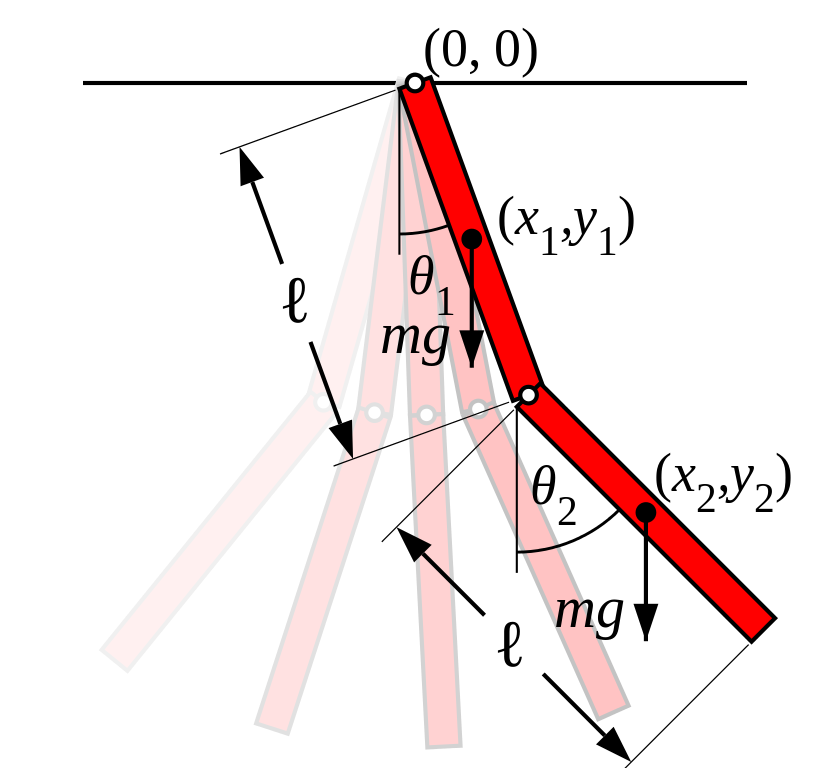
\includegraphics[height=4cm]{Double-compound-pendulum.png}

The dynamics of a double-pendulum can be descibed with the following equations 
( This example was copied from https://en.wikipedia.org/wiki/Double\_pendulum )

variables $\theta_1, \theta_2, p_{\theta_1}, p_{\theta_2}$:
\begin{eqnarray}
   \frac{d \theta_1}{dt}= \frac{6}{m l^2} \frac{2 p_{\theta_1} - 3cos(\theta_1-\theta_2) p_{\theta_2}}
   {16-9 cos^2(\theta_1-\theta_2)}\\
   \frac{d \theta_2}{dt}= \frac{6}{m l^2} \frac{8 p_{\theta_2} - 3cos(\theta_1-\theta_2) p_{\theta_1}}
   {16-9 cos^2(\theta_1-\theta_2)}\\
   \frac{dp_{\theta_1}}{dt} = -\frac{1}{2} ml^2 \left( \frac{d \theta_1}{dt} \frac{d \theta_2}{dt} sin(\theta_1-\theta_2) + 3\frac{g}{l} sin(\theta_1) \right)  \\
   \frac{dp_{\theta_1}}{dt} = -\frac{1}{2} ml^2 \left( -\frac{d \theta_1}{dt} \frac{d \theta_2}{dt} sin(\theta_1-\theta_2) + \frac{g}{l} sin(\theta_2) \right) 
\end{eqnarray}
where the $x,y$-position of the middle of the two segments can be computed as:
\begin{eqnarray}
   x_1 = \frac{l}{2} sin(\theta_1) \\
   y_1 = \frac{-l}{2} cos(\theta_1) \\
   x_2 = l ( sin(\theta_1) + \frac{1}{2} sin(\theta_2) ) \\
   y_2 = -l ( cos(\theta_1) + \frac{1}{2} cos(\theta_2) )
\end{eqnarray}

This model, although simple, is very nonlinear and has a chaotic nature.  Its
solution is very sensitive to the parameters and the initial conditions: a
small difference in those values can lead to a very different solution.

The purpose of this exercise is to get you started with OpenDA. You will learn
to run a model in OpenDA, make modifications to the input files and plot the
results.

\begin{itemize}
\item The input for this exercise is located in directory \texttt{ exercise\_pendulum\_part1}.
      For Linux and Mac OS X, go to this directory and start \texttt{ oda\_run.sh}, the
      main application of OpenDA. For Windows, start the main application with 
      \texttt{ oda\_run\_gui.bat} from the \texttt{ \$OPENDA/bin} directory. The main 
      application allows you to view and edit the OpenDA configuration files, run your
      simulations and visualize the results.
\item Try to run a simulation with the double pendulum model. You can use the
      configuration file \texttt{ simulation\_unperturbed.oda}. 
      
      For postprocessing in Matlab the results are written to \\ \texttt{ simulation\_unperturbed\_results.m}.
      Next start Matlab and load the results. We have added a routine \texttt{ plot\_movie} to create an intuitive
      representation of the data. Please type (or copy-paste):
      \begin{lstlisting}[language=Matlab,frame=single,caption={Matlab}]
      [t,unperturbed,tobs,obs]= ...
      load_results('simulation_unperturbed_results');
      plot_movie(t,unperturbed)
      \end{lstlisting}
      
      For postprocessing in Python the results are written to \\ \texttt{ simulation\_unperturbed\_results.py}.
      These results can be loaded with:
      \begin{lstlisting}[language=Python,frame=single,caption={Python initialize}]
      import simulation_unperturbed_results as unperturbed
      # use reload(unperturbed) if unperturbed was loaded before
      \end{lstlisting}
      We have added a routine \texttt{ plot\_movie} to create an intuitive
      representation of the data. 
      \begin{lstlisting}[language=Python,frame=single,caption={Python}]
      import pendulum as p #needed only once
      p.plot_movie(unperturbed.model_time,unperturbed.x)
      \end{lstlisting}
      
      To create a time-series plot in Matlab type:
      \begin{lstlisting}[language=Matlab,frame=single,caption={Matlab}]
       subplot(2,1,1);
       plot(t,unperturbed(1,:),'b-');
       ylabel('\theta_1');
       subplot(2,1,2);
       plot(t,unperturbed(2,:),'b-');
       ylabel('\theta_2');
       xlabel('time');
      \end{lstlisting}
      
      To create a time-series plot in Python type:
      \begin{lstlisting}[language=Python,frame=single,caption={Python}]
      plt.subplot(2,1,1)
      plt.plot(unperturbed.model_time,unperturbed.x[:,0],'b') #python counts starting at 0
      plt.ylabel(r'$\theta_1$') # use raw string and latex for label
      plt.subplot(2,1,2)
      plt.plot(unperturbed.model_time,unperturbed.x[:,1],'b')
      plt.ylabel(r'$\theta_2$')
      plt.show() #only needed if interactive plotting is off. Set with plt.ioff(), plt.ion()
      \end{lstlisting}
%


\item Then you can start an alternative simulation with the double-pendulum model that
       starts with a slightly different initial condition using the
       configuration file \texttt{ simulation\_perturbed.oda}. The different initial conditions
       can be found in \texttt{model\/DoublePendulumStochModel.xml} and \\
       \texttt{model\/DoublePendulumStochModel\_perturbed.xml}

\item  Visualize the unperturbed and perturbed results in a single plot. Make
       a movie and a time-series plot of $\theta_1$ and $\theta_2$ variables. Do you see
       the solutions diverging like the theory predicts?
       
      \begin{lstlisting}[language=Matlab,frame=single,caption={Matlab}]
       [tu,unperturbed,tobs1,obs1]=load_results('simulation_unperturbed_results');
       [tp,perturbed,tobs2,obs2]=load_results('simulation_perturbed_results');
       figure(1);clf;subplot(2,1,1);
       plot(tu,unperturbed(1,:),'b');
       hold on;
       plot(tp,perturbed(1,:),'g');
       hold off;
       legend('unperturbed','perturbed')
       subplot(2,1,2);
       plot(tu,unperturbed(2,:),'b');
       hold on;
       plot(tp,perturbed(2,:),'g');
       hold off;
      \end{lstlisting}
      
      To create a movie with both results in python type:
      \begin{lstlisting}[language=Python,frame=single,caption={Python initialize}]
      import simulation_unperturbed_results as unperturbed
      import simulation_perturbed_results as perturbed
      p.plot_movie(unperturbed.model_time,unperturbed.x,perturbed.x)
      \end{lstlisting}

      To create a time-series plot with both results in Python type:
      \begin{lstlisting}[language=Python,frame=single,caption={Python}]
      plt.subplot(2,1,1)
      plt.plot(unperturbed.model_time,unperturbed.x[:,0],'b') #python counts starting at 0
      plt.plot(perturbed.model_time,perturbed.x[:,0],'g') #python counts starting at 0
      plt.ylabel(r'$\theta_1$') # use raw string and latex for label
      plt.subplot(2,1,2)
      plt.plot(unperturbed.model_time,unperturbed.x[:,1],'b')
      plt.plot(perturbed.model_time,perturbed.x[:,1],'g')
      plt.ylabel(r'$\theta_2$')
      plt.show() 
      \end{lstlisting}
      
\item Next we want to create an ensemble of model runs all with slightly different initial conditions. 
      You can do this in a number of steps:
      \begin{itemize}
      \item First create the input file \texttt{ simulation\_ensemble.oda} based on\\
            \texttt{ simulation\_unperturbed.oda}. Change the algorithm and the
            configuration of the algorithm.\\
            hint: the algorithm is called \\
            org.openda.algorithms.kalmanFilter.SequentialEnsembleSimulation.
      \item Create a configuration file for the Ensemble algorithm (e.g. named
            \texttt{ algorithm/SequentialEnsembleSimulation.xml}) with the following content:
      \begin{lstlisting}[language=XML,frame=single,caption={XML-input for sequentialAlgorithm}]
      <?xml version="1.0" encoding="UTF-8"?>
      <sequentialAlgorithm>
         <analysisTimes type="fromObservationTimes" ></analysisTimes>
         <ensembleSize>5</ensembleSize>
         <ensembleModel stochParameter="false"
                        stochForcing="false"
                        stochInit="true" />
      </sequentialAlgorithm>
      \end{lstlisting}
      Hint: do not forget to reference \texttt{ algorithm/SequentialEnsembleSimulation.xml} in \\ \texttt{ simulation\_ensemble.oda}
      and do not forget to give a diferent name to the output files.
      \item Run the new configuration with OpenDA.

      \item make a plot of the first and second variable of the five ensemble
      members in a single time-series plot
      \begin{lstlisting}[language=Matlab,frame=single,caption={Matlab}]
      [t,ens]=load_ensemble('simulation_ensemble_results');
      ens_th1=reshape(ens(1,:,:),size(ens,2),size(ens,3));
      ens_th2=reshape(ens(2,:,:),size(ens,2),size(ens,3));
      clf; subplot(2,1,1);
      plot(t(2:end),ens_th1);
      ylabel('\theta_1');
      subplot(2,1,2);
      plot(t(2:end),ens_th2);
      ylabel('\theta_2');
      xlabel('time');
      \end{lstlisting}
      
      \begin{lstlisting}[language=Python,frame=single,caption={Python}]
      import ensemble
      import simulation_ensemble_results as res
      (t,ens)=ensemble.reshape_ensemble(res)
      ens1=ens[:,0,:] #note we start counting at 0
      ens2=ens[:,1,:]
      plt.subplot(2,1,1)
      plt.plot(t[1:],ens1,'b')
      plt.ylabel(r'$\theta_1$')
      plt.subplot(2,1,2)
      plt.plot(t[1:],ens2,'b')
      plt.ylabel(r'$\theta_2$')
      plt.show()
      \end{lstlisting}
      
      \item Observations of $\theta_1$ and $\theta_2$ are available as well. Make a plot of
      the observations together with the simulation results.
      \begin{lstlisting}[language=Matlab,frame=single,caption={Matlab}]
	[t,unperturbed,tobs,obs]= ...
	load_results('simulation_unperturbed_results');
       subplot(2,1,1);
       plot(t,unperturbed(1,:),'b-');
       hold on
       plot(tobs,obs(1,:),'k+');
       hold off
       ylabel('\theta_1');
       subplot(2,1,2);
       plot(t,unperturbed(2,:),'b-');
       hold on
       plot(tobs,obs(2,:),'k+');
       hold off
       ylabel('\theta_2');
       xlabel('time');
      \end{lstlisting}
      \begin{lstlisting}[language=Python,frame=single,caption={Python}]
      import simulation_unperturbed_results as unperturbed
      plt.subplot(2,1,1)
      plt.plot(unperturbed.model_time,unperturbed.x[:,0],'b') #python counts starting at 0
      plt.plot(unperturbed.analysis_time,unperturbed.obs[:,0],'k+') #python counts starting at 0
      plt.ylabel(r'$\theta_1$') # use raw string and latex for label
      plt.subplot(2,1,2)
      plt.plot(unperturbed.model_time,unperturbed.x[:,1],'b')
      plt.plot(unperturbed.analysis_time,unperturbed.obs[:,1],'k+')
      plt.ylabel(r'$\theta_2$')
      plt.show()
      \end{lstlisting}
      
      We can see that although our simulation starts on the right track, it quickly diverges from the observations.
      The aim of the Ensemble Kalman filter or data-assimilation in general, is to keep the model on track. 
      \end{itemize}

\end{itemize}
